\section{Understanding Events}
Events are fundamental linguistic elements in human speech. Thus understanding 
events is a fundamental prerequisite for deeper semantic 
analysis of language, and any computational system of human language should
have a model of events. One can view an event as an occurrence of a certain 
action caused
by an agent, affecting a patient at a certain time and place and so on. It is 
the combination of the entities
filling the said roles that define an event. Furthermore, certain combinations 
of these role fillers
agree with the general state of the world, and others do not. For example, 
consider the events described by the following
sentences.
\begin{itemize}
 \item[] \textit{Man recovering after being bitten by his dog.}
 \item[] \textit{Man recovering after being shot by cops.}
\end{itemize}
The \textit{agent} of the \textit{biting} action is \textit{dog} in the first 
sentence, and that of the \textit{shooting}
action in the second sentence is \textit{cops}. The patient in both sentences is 
\textit{man}.
Both combinations of role-fillers result in events that agree with most people's 
world view. That is not the case with
the event in the following sentence.
\begin{itemize}
 \item[] \textit{Man recovering after being shot by his dog.}
\end{itemize}
This combination does not agree with our expectations about the general state of 
affairs, and consequently one
might find this event strange. While all three sentences above are equally
valid syntactically, it 
is our knowledge about the role fillers 
---both individually and specifically in combination---  
that enables us to 
differentiate between normal and anomalous events.  Hence we hypothesize that
\emph{anomaly is a result of unexpected or 
unusual combination of semantic role fillers}.

In this chapter, we introduce the problem of automatic anomalous event
detection and propose a novel event model that can learn to differentiate
between normal
and anomalous events. We generally define anomalous events as those that are
unusual compared
to the general state of affairs and might invoke surprise when reported. An 
automatic
anomaly detection algorithm has to encode
the goodness of semantic role filler coherence.  This is a hard problem since
determining what a good combination of role fillers is 
requires deep semantic and pragmatic knowledge.  
Moreover, manual judgment of anomaly itself may be difficult and people often
may not agree with each other in this
regard.  We describe the difficulty in human judgment in greater detail in
Section~\ref{sec:nem_annot}.  
Automatic detection of anomaly requires encoding complex information, which
poses the challenge of sparsity
due to the discrete representations of meaning, that are words.  These problems
range from polysemy and synonymy at the 
lexical semantic level to entity and event coreference at the discourse level.

We define an event as the pair $(V, \textbf{A})$, where $V$
is the predicate or a semantic verb\footnote{By semantic verb, we mean an action 
word whose
syntactic category is not necessarily a verb.  
For example, in \textit{Terrorist attacks on the World Trade Center..},
\textit{attacks} is not a verb but is still an 
action word.}, and $\textbf{A}$ is the set of its semantic arguments like agent,
patient, time, location, so on. Our aim
is to obtain a vector representation of the event that is composed from
representations of individual words, while explicitly guided by the semantic
role structure. This representation can be understood as an embedding of the
event in an event space. 

\section{Related Work} \label{sec:nem_background}
Selectional preference, a notion introduced by \cite{wilks1973preference}, 
refers to the paradigm of modeling semantics of
natural language in terms of the restrictions a verb places on its arguments. 
For example, the knowledge required to identify
one of the following sentences as meaningless can be encoded as preferences (or 
restrictions) of the verb.
\begin{itemize}
 \item[] \textit{Man eats pasta.}
 \item[] \textit{Poetry eats computers.}
\end{itemize}
The restrictions include \textit{eat} requiring its subject to be animate, its 
object to be edible, and so on. Though the
notion was originally proposed for a verb and its dependents in the context of 
dependency grammars, it is equally applicable to
other kinds of semantic relations. In this work,
we use this idea in the context of verbs and their semantic role fillers.

The idea is that identifying the right sense of the word can be guided by the 
preferences of the other words it is related to.  \cite{resnik1997selectional}
illustrates this through the example of disambiguating the sense of the word 
\textit{letter} in the phrase \textit{write a letter}.
While \textit{letter} has multiple senses, as an object, the verb \textit{write} 
``prefers'' the sense closer to \textit{reading matter} more than others.
At the phrasal level, selectional preferences are useful in encoding complex 
phenomena like metaphor.  Metaphorical usage of words usually involves violating 
selectional restrictions.
For example the phrase \textit{kill an idea} is a metaphor, because 
\textit{kill} does not usually take abstract concepts as objects.  The phrase 
itself is common and
one can easily attribute a metaphorical sense to the verb kill and resolve the 
violation.  \cite{wilks2007making}, \cite{wilks2007preferential}, 
\cite{krishnakumaran2007hunting},
\cite{shutova2013statistical}, among others discuss the selectional preference 
view of metaphor identification.
Automatic acquisition of selectional preferences from text is a well studied 
problem.  \cite{resnik1996selectional} proposed the first broad coverage 
computational model of selectional preferences.  The approach is based on using 
WordNet's hierarchy to generalize across words.
It measures selectional association strength of an triple $(v, r, c)$ with verb 
$v$, relation $r$ and an argument class $c$ as the Kullback-Leibler divergence 
between the the distributions $P(c|v, r)$  $c$
and $P(c|r)$ normalized over all classes of arguments that occur with the $(v, 
r)$ pair.  \cite{abe1996learning} also use WordNet, and model selectional 
preferences by minimizing the length tree cut through
the noun hierarchy.  \cite{ciaramita2000explaining} encode the hierarchy as a 
Bayesian network and learn selectional preferences using probabilistic graphical 
methods.
\cite{rooth1999inducing} take a distributional approach, and use latent variable 
models to induce classes of noun-verb pairs, and thus learn their preferences.  
Methods by \cite{erk2007simple,erk2010flexible}
are also distributional, and have been described earlier in this paper.  
\cite{seaghdha2010latent} proposed the use of Latent Dirichlet Allocation (LDA), 
to model preferences as topics.  \cite{van2009non} used
non-negative tensor factorization, and modeled subject-verb-object triples as a 
three-way tensor.  The tensor is populated with co-occurrence frequencies, and 
the selectional preferences are measured from decomposed
representations of the three words in the triple. \cite{van2014neural} trains 
neural networks to score felicitous triples higher than infelicitous ones.

\cite{erk2010flexible} also model selectional preferences using vector spaces.  
They measure the 
goodness of the fit of a noun with a verb in terms of the similarity between the 
vector of the noun and 
some ``exemplar'' nouns taken by the verb in the same argument role.  
\cite{baroni2010distributional} 
also measure selectional preference similarly, but instead of exemplar nouns, 
they calculate a 
prototype vector for that role based on the vectors of the most common nouns 
occurring in that 
role for the given verb.  \cite{lenci2011composing} builds on this work and 
models the phenomenon
that the expectations of the verb or its role-fillers change dynamically given 
other role fillers.

% \section{Machine Learning Background} \label{sec:nem_neural_networks}
% Our model uses Recurrent Neural Networks (RNN) with Long Short-Term Memory (LSTM)
% \citep{hochreiter1997long} cells. We describe the relevant technical details here.
% RNNs, as opposed to feed-forward neural networks are networks with loops in them

\section{Data}
We crawl 3684 ``weird news'' headlines available publicly 
on the website of NBC
news\footnote{\url{
http://www.nbcnews.com/html/msnbc/3027113/3032524/4429950/4429950_1.html}}, 
such as the following: 
\begin{itemize}
 \item[] \textit{India weaponizes world's hottest chili.}
 \item[] \textit{Man recovering after being shot by his dog.}
 \item[] \textit{Thai snake charmer puckers up to 19 cobras.}
\end{itemize}
We assume that the events extracted from this source, called NBC Weird Events
(NWE) henceforth, are
anomalous for training.  NWE contains 4271 events extracted using 
SENNA's SRL.  We use 3771 of those events as our negative training data. 
Similarly, we extract events also from
headlines in the AFE section of Gigaword, called Gigaword Events (GWE)
henceforth.  We assume these events are normal.
To use as positive examples for training event composition, we sample roughly
the same number of events from 
GWE as our negative examples from NWE. From the two sets, we uniformly sample 
1003 events
as the test set and validate the labels by getting crowd-sourced annotations.

\subsection{Annotation}
\label{sec:nem_annot}
We post the annotation of the test set containing 1003 events as
Human Intelligence Tasks (HIT) on Amazon Mechanical Turk (AMT).
We break the task into 20 HITs and ask the workers to select one of the 
four options - \textit{highly unusual}, \textit{strange}, \textit{normal} and 
\textit{cannot say} for each event.  We ask them to select \textit{highly
unusual} when the 
event seems too strange to be true, \textit{strange} if it seems unusual but 
still plausible, and \textit{cannot say} only if the information present in the 
event is not sufficient to make a decision.  We publicly release this set of 
1003
annotated events for evaluating future research.

\begin{table}
\begin{center}
  \begin{tabular}[c]{|c|c|}
 \hline
  Total number of annotators & 22\\
  \hline
  \textit{Normal} annotations & 56.3\% \\
  \hline
  \textit{Strange} annotations & 28.6\% \\
  \hline
  \textit{Highly unusual} annotations & 10.3\% \\
  \hline
  \textit{Cannot Say} annotations & 4.8\% \\
  \hline
  Avg. events annotated per worker & 344 \\
  \hline
  4-way Inter annotator agreement ($\alpha$) & 0.34 \\
  \hline
  3-way Inter annotator agreement ($\alpha$) & 0.56 \\
  \hline
  \end{tabular}
\end{center}
 \caption{Annotation Statistics}
 \label{table:annot}
\end{table}
Table~\ref{table:annot} shows some statistics of the annotation task.  We
compute the Inter Annotator
Agreement (IAA) in terms of Kripendorff's alpha \cite{krippendorff1980content}. 
The advantage of using this
measure instead of the more popular Kappa is that the former can deal with
missing information, which is the case with
our task since annotators work on different overlapping subsets of the test set.
 The 4-way IAA shown in the table 
corresponds to agreement over the original 4-way decision (including
\textit{cannot say}' while the 3-way IAA is measured after merging the 
\textit{highly unusual} and \textit{strange} decisions.  

Additionally we use
MACE \cite{hovy2013learning} to assess the quality of 
annotation.  MACE models the annotation task as a generative process of
producing the observed labels conditioned on the 
true labels and the competence of the annotators, and predicts both the latent
variables.  The average of competence of annotators, 
a value that ranges from 0 to 1, for our task is 0.49 for the 4-way decision and
0.59 for the 3-way decision.  

We generate
true label predictions produced by MACE, discard the events for which the
prediction remains to be \textit{cannot say}, and use the 
rest as the final labeled test set.  This leaves 949 events as our test dataset,
of which only 41\% of the labels are \textit{strange} or \textit{highly
unusual}.  It has to be noted that even though our test set 
has equal size samples from both NWE and GWE, the true distribution is not
uniform.

\subsection{Language Model Separability}
Given the annotations, we test to see if the
sentences corresponding to anomalous events can be separated from normal events 
by simpler 
features.  We build a n-gram language model from the training data set used for 
argument composition and 
measure the perplexity of the sentences in the test set.  
Figure~\ref{fig:nem_lm_ppl} shows
a comparison of the perplexity scores for different labels. If the n-gram 
features are enough 
to separate different classes of sentences, one would expect the sentences 
corresponding to 
\textit{strange} and \textit{highly unusual} labels to have higher perplexity 
ranges than \textit{normal}
sentences, because the language model is built from a dataset that is expected 
to have a distribution of
sentences where majority of them contain normal events.  As it can be seen in 
Figure~\ref{fig:nem_lm_ppl}, 
except for a few outliers, most data points in all the categories are in similar 
perplexity ranges.
Hence, sentences with different labels cannot be separated based on an n-gram 
language model features.

\begin{figure}
  \begin{center}
  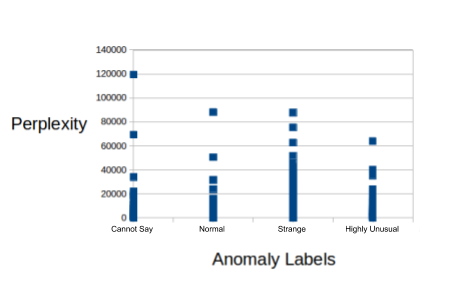
\includegraphics[width=4in]{figures/perplexity-comparison.png}
  \caption{Comparison of perplexity scores for different labels}
  \label{fig:nem_lm_ppl}
  \end{center}
\end{figure}

\section{Model for Semantic Anomaly Detection}
Neural Event Model (NEM) is a supervised model that learns to differentiate between anomalous and
normal events by 
classifying dense representations of events, otherwise known as event embeddings. We treat the problem as a binary classification problem, with
\textit{normal} and \textit{anomalous} being the two classes.
The event embeddings are computed using a structured composition model
that represents an event as the composition of the five slot-fillers: \textbf{action},
\textbf{agent}, \textbf{patient}, \textbf{time} and \textbf{location}.
Figure~\ref{fig:nem} shows the pipeline for anomalous event detection using NEM. We
first identify the fillers for the five slots mentioned above, by running a PropBank \citep{palmer2005proposition}
style Semantic Role Labeler (SRL). We use the following mapping of roles to obtain the event structure:
\begin{itemize}
 \item V $\rightarrow$ action
 \item A0 $\rightarrow$ agent
 \item A1 $\rightarrow$ patient
 \item AM-TMP $\rightarrow$ time
 \item AM-LOC $\rightarrow$ location
\end{itemize}
This structured input is then passed to NEM. The model has three components:

\paragraph{Argument Composition} This component encodes all the role fillers as vectors in the same space.
This is accomplished by embedding the words in each role filler, and then passing them through a Recurrent
Neural Network (RNN) with Long Short-Term Memory (LSTM) \citep{hochreiter1997long} cells. Note that the same LSTM is
used for all the slots. Concretely,
\begin{equation}
 a_s = \text{LSTM}(I_s)
\end{equation}
where $I_s$ denotes the ordered set of word vector representations in in the filler of slot $s$, and
$a_s$ represents the vector representation of that slot filler.

\paragraph{Event Composition} The slot filler representations are then composed using slot specific
projection weights to obtain a single event representation. Concretely,
\begin{align}
 \bar{a}_s &= \tanh(W_s^\intercal a_s + b_s) \quad \text{where } s \in \{c,g,p,t,l\} \\
 e &=  \bar{a}_c + \bar{a}_g + \bar{a}_p + \bar{a}_t + \bar{a}_l 
\end{align}
$W_s \in \mathbb{R}^{d \times d}$ and $b_s \in \mathbb{R}^{d}$ are slot specific projection weights and biases respectively, with $s$ denoting one of a\underline{c}tion,
a\underline{g}ent, \underline{p}atient, \underline{t}ime and \underline{l}ocation. $d$ is the dimensionality of the word embeddings.
Event composition involves performing non-linear projections of all slot-filler representations, and finally obtaining an event representation
$e$.

\paragraph{Anomaly Classification} The event representation is finally passed through a softmax layer to obtain
the predicted probabilities for the two classes.
\begin{align}
 p_e & = \text{softmax}(W_e^\intercal e + b_e) \\
\end{align}
$W_e \in \mathbb{R}^{d \times 2}$ and $b_e \in \mathbb{R}^2$ are the weight and bias values of the softmax layer respectively.
As it can be seen, the layer projects the event representation into a two-dimensional space before applying the softmax non-linearity.

\begin{figure}
  \begin{center}
  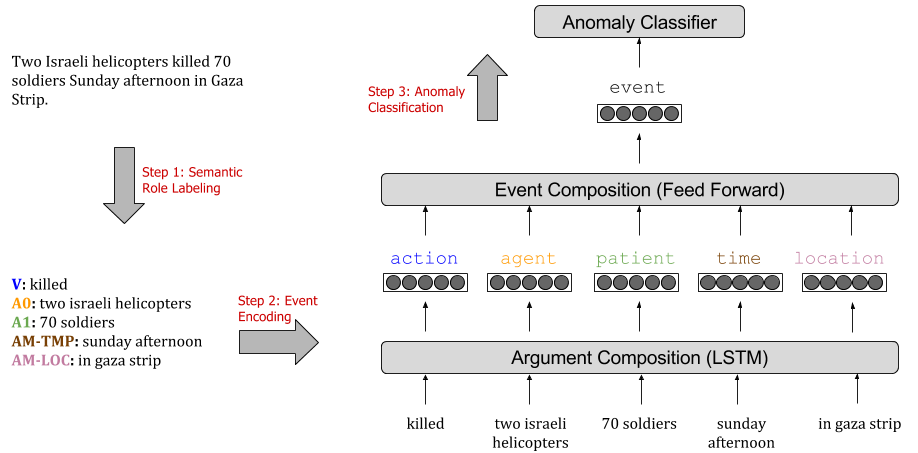
\includegraphics[width=6.5in]{figures/nem_pipeline.png}
  \caption{Anomaly Classification Pipeline with Neural Event Model}
  \label{fig:nem}
  \end{center}
\end{figure}

\subsection{Training}
Given the output from NEM, we define
\begin{align}
 p^1_e(\theta) &= P(\text{anomalous} | e; \theta) \\
 p^0_e(\theta) &= P(\text{normal} | e; \theta)
\end{align}
where $\theta$ are the parameters in the model and compute the label loss based on the prediction at the end of anomaly classification as a cross entropy loss as follows:
\begin{equation}
J(\theta) = - l \log p^1_e(\theta) + (1-l) \log p^0_e(\theta)
\end{equation}
where $l$ is the reference binary label indicating whether the event is normal or
anomalous. The three components of the model described above: argument composition, event composition and anomaly classification are all trained jointly.
That is, we optimize the following objective.
\begin{equation}
 \theta^* = \argmin_{\theta} J(\theta)
\end{equation}
where $\theta$ includes all $W_s$ and $b_s$ from all the slots, $W_e$ and $b_e$ from event composition and also all the LSTM parameters from argument composition.
We optimize this objective using ADAM \citep{kingma2014adam}. The model is implemented\footnote{The code is publicly available at \url{https://github.com/pdasigi/neural-event-model}}
using Keras \citep{chollet2015keras}. Note that the model described here is an extension of the one described in our previously published paper \citep{dasigi2014modeling}.
The main improvements here include using an LSTM-RNN as the encoder in argument composition instead of a simple RNN, and jointly training argument composition, event composition and anomaly classification,
whereas the older model included training argument composition separately using an unsupervised objective.

\section{Results}
We merged the two anomaly classes (strange and highly unusual) and calculated accuracy and F-score (for the anomaly class) of the binary
classifier. For the sake of comparison, we also define the following two baseline models.

\paragraph{PMI Baseline} We compare the performance of our model against a baseline that is based
on how well the semantic arguments in the event match the selectional preferences 
of the predicate.  We measure selectional preference using Point-wise Mutual Information
(PMI) \cite{church1990word} of the head words of each semantic argument with the predicate.  
The baseline model is built as follows.  We perform dependency parsing using MaltParser
\cite{nivre2007maltparser} on the sentences in the training data used in the first phase of training to
obtain the head words of the semantic arguments.  We then calculate the PMI values of all the pairs
$<h_A, p>$ where $h$ is the head word of argument $A$ and $p$ is the predicate of the event.  
For training our baseline classifier, we use the labeled training data from the event composition phase.
The features to this classifier are the PMI measures of the $<h_A, p>$ pairs estimated from the larger
dataset.  The classifier thus trained to distinguish between anomalous and normal events is applied to the test set.

\paragraph{LSTM Baseline} To investigate the importance of our proposed event representation, we also implemented a LSTM baseline that
directly encodes sentences. The following equations describe the model.
\begin{align}
 w &= \text{LSTM}(I) \\
 \bar{w} &= \tanh(W_w^\intercal w + b_w) \\
 p_u &= \text{softmax}(W_u^\intercal \bar{w} + b_u)
\end{align}
Note that this model is comparable in complexity, and has the same number of non-linear transformations as NEM. $\bar{w}$ represents a
word level composition instead of an argument-level composition in NEM, and $p_u$ is a probability distribution defined over an
\underline{u}nstructured composition as features. Training of this baseline model is done in the same way as NEM.

\begin{table}
\begin{center}
  \begin{tabular}[c]{|c|c|c|}
 \cline{2-3}
 \multicolumn{1}{c|}{}& \textbf{Accuracy} & \textbf{F-Score} \\
 \hline
 PMI Baseline& 45.2\% & 45.1\%\\
 LSTM Baseline & 82.5\% & 77.4\%\\
 \hline
 NEM & \textbf{84.9\%}& \textbf{79.7\%}\\
 \hline
  \end{tabular}
\end{center}
 \caption{Classification Performance and Comparison with Baselines}
 \label{table:nem_anomaly_results}
\end{table}

Table~\ref{table:nem_anomaly_results} shows the results and a comparison with the two baselines.  The accuracy of the 
baseline classifier is lower than 50\%, which is the expected accuracy of a classifier that assigns labels randomly.  
As seen in the table, the LSTM model proves to be a strong baseline, but it under performs in comparison with NEM,
showing the value of our proposed event composition model. The difference between the performance of
NEM and the LSTM baseline is statistically significant with $p < 0.0001$. Figure~\ref{fig:nem_roc} shows the ROC curves
for NEM and the LSTM baseline.
\begin{figure}
  \begin{center}
  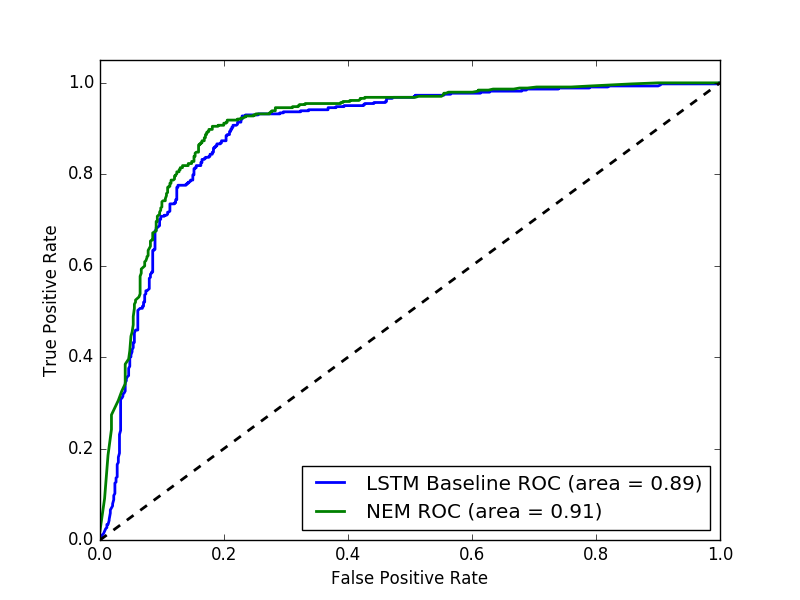
\includegraphics[width=4in]{figures/nem_roc.png}
  \caption{ROC curves for the LSTM baseline and NEM}
  \label{fig:nem_roc}
  \end{center}
\end{figure}


To further compare NEM with human annotators, we give to MACE, the binary predictions produced
by NEM, and those by the LSTM baseline along with the annotations and
measure the competence.  For the sake of comparison, we also give to MACE, a list of
random binary labels as one of the annotations 
to measure the competence of a hypothetical worker that made random choices. 
These results are reported in Table~\ref{table:nem_mace_competence}.
\begin{table}
\begin{center}
  \begin{tabular}[c]{|c|c|}
 \hline
 Human highest  & 0.896 \\
  Human average & 0.633 \\
  Human lowest & 0.144 \\
  \hline
  Random & 0.054 \\
  \hline
  LSTM Baseline & 0.743 \\
  NEM &  0.797 \\
  \hline
  \end{tabular}
\end{center}
 \caption{Anomaly Detection Competence}
 \label{table:nem_mace_competence}
\end{table}
Unsurprisingly, the competence of the random classifier is very low, and is worse than the least competent human.
It can be seen that MACE predicts both the LSTM baseline and NEM to be more competent than human average. This is an encouraging
result, especially given that this is a hard problem even for humans.

\section{Discussion}
%TODO: Error analysis
One important aspect of anomaly that is currently not handled by NEM
is the level of generality of the concepts the events contain.  Usually
more general concepts cause events to be more normal since they convey
lesser information.  For example, an American soldier shooting another American
soldier
may be considered unusual, while a soldier shooting another soldier may not be
as unusual, and at the 
highest level of generalization, a person shooting another person is normal. 
This information
of generality has to be incorporated into the event model.  This can be achieved
by integrating 
real world knowledge from knowledge bases like Wordnet \cite{miller1995wordnet}
or from corpus 
statistics like the work by \cite{lin1998automatic} into the event model.  
\cite{bordes2011learning} learn continuous representations of 
entities and relations in knowledge bases.  More recently, an alternative approach
for doing the same was proposed by \cite{chen2013learning}.  These representations
can greatly help modeling events.

Finally, the idea of modeling event composition can help processing event data
in general and can 
be applied to other tasks like finding co-referent events.